% В этом документе преамбула

\documentclass[a4paper,12pt]{article}

\usepackage{lscape} % горизонтальный режим
\usepackage{pdflscape}

\usepackage{lipsum} % тестовые тексты

%%% Работа с русским языком
\usepackage{cmap}					% поиск в PDF
\usepackage{mathtext} 				% русские буквы в формулах
\usepackage[T2A]{fontenc}			% кодировка
\usepackage[utf8]{inputenc}			% кодировка исходного текста
\usepackage[english,russian]{babel}	% локализация и переносы
\usepackage{indentfirst}			% чтобы первый абзац в разделе отбивался красной строкой
\frenchspacing						% тонкая настройка пробелов
\usepackage{gensymb}				% символы по типу градусов
\usepackage{algorithm}				% для алгоритмов
\usepackage{algorithmic}			% для алгоритмов

%%% Приведение начертания букв и знаков к русской типографской традиции
\renewcommand{\epsilon}{\ensuremath{\varepsilon}}
\renewcommand{\phi}{\ensuremath{\varphi}}			% буквы "эпсилон"
\renewcommand{\kappa}{\ensuremath{\varkappa}}		% буквы "каппа"
\renewcommand{\le}{\ensuremath{\leqslant}}			% знак меньше или равно
\renewcommand{\leq}{\ensuremath{\leqslant}}			% знак меньше или равно
\renewcommand{\ge}{\ensuremath{\geqslant}}			% знак больше или равно
\renewcommand{\geq}{\ensuremath{\geqslant}}			% знак больше или равно
\renewcommand{\emptyset}{\varnothing}				% знак пустого множества

%%% Дополнительная работа с математикой
\usepackage{amsmath,amsfonts,amssymb,amsthm,mathtools,esint} % AMS
\usepackage{wasysym}
\usepackage{icomma} % "Умная" запятая: $0,2$ --- число, $0, 2$ --- перечисление

%% Номера формул
\mathtoolsset{showonlyrefs=true} % Показывать номера только у тех формул, на которые есть \eqref{} в тексте.

%% Свои команды

% операции, не определённые (или имеющие иные обохначения) в мат. пакетах
\DeclareMathOperator{\sgn}{\mathop{sgn}}				% ф-ия sgn
\renewcommand{\tg}{\mathop{\mathrm{tg}}\nolimits}		% обозначение тангенса

%% Перенос знаков в формулах (по Львовскому)
\newcommand*{\hm}[1]{#1\nobreak\discretionary{}
{\hbox{$\mathsurround=0pt #1$}}{}}

%%% Работа с картинками
\usepackage{graphicx}  				% Для вставки рисунков
\graphicspath{{images/}{images2/}}  % папки с картинками
\setlength\fboxsep{3pt} 			% Отступ рамки \fbox{} от рисунка
\setlength\fboxrule{1pt} 			% Толщина линий рамки \fbox{}
\usepackage{wrapfig} 				% Обтекание рисунков текстом

%%% Работа с таблицами
\usepackage{array,tabularx,tabulary,booktabs} 	% Дополнительная работа с таблицами
\usepackage{longtable}  						% Длинные таблицы
\usepackage{multirow}							% Слияние строк в таблице

%%% Теоремы

\newtheoremstyle{break}% name
	{}%         Space above, empty = `usual value'
	{}%         Space below
	{\itshape}% Body font
	{}%         Indent amount (empty = no indent, \parindent = para indent)
	{\bfseries}% Thm head font
	{.}%        Punctuation after thm head
	{\newline}% Space after thm head: \newline = linebreak
	{}%         Thm head spec
\theoremstyle{break}

% \theoremstyle{plain} % Стиль по умолчанию
\newtheorem{theorem}{Теорема}[section]
\newtheorem{lemma}{Лемма}[section]
\newtheorem{definition}[theorem]{Определение}
\newtheorem{property}{Свойство}
 
\newtheorem{corollary}{Следствие}[theorem]

\newtheoremstyle{example}	% style name
	{2ex}					% above space
	{2ex}					% below space
	{}						% body font
	{}						% indent amount
	{\bf}				% head font
	{.}						% post head punctuation
	{\newline}				% post head punctuation
	{\thmname{#1}\thmnumber{ #2}\thmnote{ (#3)}}						% head spec

\theoremstyle{example}
\newtheorem{exmp}{Пример}[section]
 
\theoremstyle{remark} % "Примечание"
\newtheorem*{nonum}{Решение}
\newtheorem*{evidence}{Доказательство}
\newtheorem*{remark}{Примечание}

%%% Программирование
\usepackage{etoolbox} % логические операторы

%%% Страница
\usepackage{extsizes} % Возможность сделать 14-й шрифт
\usepackage{geometry} % Простой способ задавать поля
	\geometry{top=15mm}
	\geometry{bottom=35mm}
	\geometry{left=10mm}
	\geometry{right=10mm}

%\usepackage{fancyhdr} % Колонтитулы
% 	\pagestyle{fancy}
 	%\renewcommand{\headrulewidth}{0pt}  % Толщина линейки, отчеркивающей верхний колонтитул
% 	\lfoot{Нижний левый}
% 	\rfoot{Нижний правый}
% 	\rhead{Верхний правый}
% 	\chead{Верхний в центре}
% 	\lhead{Верхний левый}
%	\cfoot{Нижний в центре} % По умолчанию здесь номер страницы

\usepackage{setspace} % Интерлиньяж (межстрочные интервалы)
%\onehalfspacing % Интерлиньяж 1.5
%\doublespacing % Интерлиньяж 2
%\singlespacing % Интерлиньяж 1

\usepackage{lastpage} % Узнать, сколько всего страниц в документе.

\usepackage{soulutf8} % Модификаторы начертания

\usepackage{hyperref}
\usepackage[usenames,dvipsnames,svgnames,table,rgb]{xcolor}
\hypersetup{				% Гиперссылки
    unicode=true,           % русские буквы в раздела PDF
    pdftitle={Заголовок},   % Заголовок
    pdfauthor={Автор},      % Автор
    pdfsubject={Тема},      % Тема
    pdfcreator={Создатель}, % Создатель
    pdfproducer={Производитель}, % Производитель
    pdfkeywords={keyword1} {key2} {key3}, % Ключевые слова
    colorlinks=true,       	% false: ссылки в рамках; true: цветные ссылки
    linkcolor=MidnightBlue, % внутренние ссылки
    citecolor=black,        % на библиографию
    filecolor=magenta,      % на файлы
    urlcolor=blue           % на URL
}

\usepackage{csquotes} % Еще инструменты для ссылок

%\usepackage[style=authoryear,maxcitenames=2,backend=biber,sorting=nty]{biblatex}

\usepackage{multicol} % Несколько колонок

%%% Работа с графикой
\usepackage{tikz}
\usetikzlibrary{calc}
\usepackage{tkz-euclide}
\usetikzlibrary{arrows}
\usepackage{pgfplots}
\usepackage{pgfplotstable}

%%% Настройка подписей к плавающим объектам
% \usepackage{floatrow}	% размещение
\usepackage{caption}	% начертание
\captionsetup[figure]{labelfont=bf,textfont=it,font=footnotesize}	% нумерация и надпись курсивом
% для подфигур: заголовок подписи полужирный, текст заголовка обычный
% выравнивание является неровным (т.е. выровненным по левому краю)
% singlelinecheck = off означает, что настройка выравнивания используется, даже если заголовок имеет длину только одну строку.
% если singlelinecheck = on, то заголовок всегда центрируется, когда заголовок состоит только из одной строки.
\captionsetup[subfigure]{labelfont=bf,textfont=normalfont,singlelinecheck=off,justification=raggedright}

%%% Stuff для листинга
\usepackage{listings}
\usepackage{xcolor}

\colorlet{mygray}{black!30}
\colorlet{mygreen}{green!60!blue}
\colorlet{mymauve}{red!60!blue}

\lstset{
	backgroundcolor=\color{gray!10},  
	basicstyle=\ttfamily,
	columns=fullflexible,
	breakatwhitespace=false,      
	breaklines=true,                
	captionpos=b,                    
	commentstyle=\color{mygreen}, 
	extendedchars=true,              
	frame=single,                   
	keepspaces=true,             
	keywordstyle=\color{blue},      
	language=c++,                 
	numbers=none,                
	numbersep=5pt,                   
	numberstyle=\tiny\color{blue}, 
	rulecolor=\color{mygray},        
	showspaces=false,               
	showtabs=false,                 
	stepnumber=5,                  
	stringstyle=\color{mymauve},    
	tabsize=3,                      
	title=\lstname                
}

% для извращённых начертаний
\usepackage{mathrsfs}

\usepackage{makecell}
\setcellgapes{3pt}

% Зачёркивание символов
\usepackage{cancel}

% перечисления с буквами
\usepackage{enumitem}

\begin{document}

\section{Организация и планирование}

\subsection{02.09.20 - способы организации производственного процесса во времени}

\begin{figure}[h]
	\center{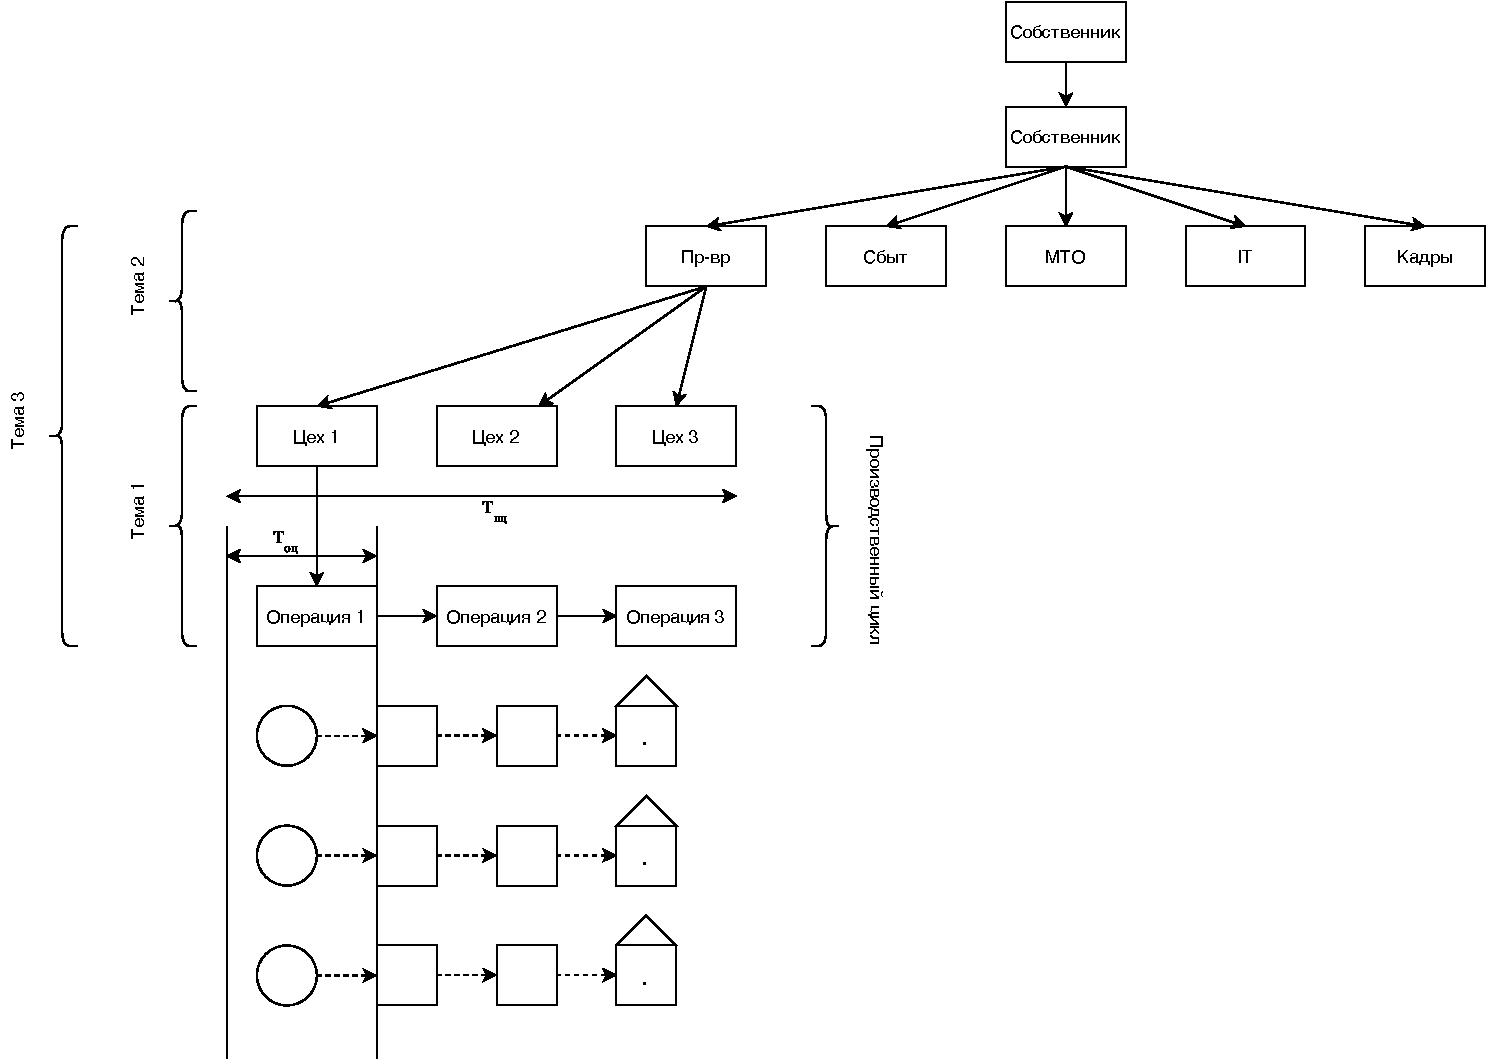
\includegraphics[scale=0.7]{./media/scheme_02_09.pdf}}
\end{figure}

\begin{remark}
	Стр. 15-16 методички
\end{remark}

Совокупность операций, необходимых для производства одного изделия - производственный цикл.

Календарный период от момента поступления сырья до момента выхода готовой продукции - длительность производственного цикла.

\noindent\textbf{Этапы изготовления: }

\begin{enumerate}
	\item Основные операции - те, которые выполняются над изделием и добавляют ему ценность. 
	\item Вспомогательные операции - не добавляют ценности, но добавляют стоимости. Например, транспортные расходы.
	\item Естественные процессы - например, покрыли плату лаком - ей нужно высохнуть.
	\item Перерывы.
\end{enumerate}

Шесть способов сокращения производственного цикла (рассматриваем характеристику времени):

\begin{enumerate}
	\item Заменить естественные процесс искусственным, например, отправить плату, покрытую лаком, в сушильную машину.
	\item Оптимизация вспомогательных операций.
	\item Совершенствование технологии производства (например, способ нанесения лака).
	\item Совмещение перерывов с естественными процессами. Использование \textit{рациональных способов сопряжения операций}.
	\item Научная организация труда на рабочем месте. Формализация того, как, например, лежат инструменты, стандартизация.
	\item Введение сменности.
\end{enumerate}

\begin{remark}
	Перерывы убрать нельзя - из устанавливает государство.
\end{remark}

Длительность операционного цикла:

\[ \text{Т}_{\text{оц}} = \frac{n_{\text{Т}_{\text{шт.}}}}{C} \]

$C$ - кол-во рабочих мест, $\text{Т}_{\text{оц}}$ - время, $\text{Т}_{\text{шт.}}$ - $t$-штучная.

\subsubsection{Рациональные способы сопряжения}

Пусть есть партия из $n = 5$ деталей, $m = 3, t_1 = 1 \text{ мин}, t_3 = 3 \text{ мин.}, t_3 = 2 \text{ мин}$.

\begin{remark}
	Рисунки и схемы см. на 18 стр. методички.
\end{remark}

\[
\text{Т}_{\text{посл.}} = n \sum_{i=1}^{m} t_i; ~~~ T_{\text{посл.} = 5 \cdot (1 + 3 + 2) = 30}
\]

Решение ускорения - "распрараллеливание"\,.

$p = 1$ - передаточая партия - количество деталей, передающихся на следующую операцию как единое целое.

\[
\text{Т}_{\text{пар.} = p \sum\limits_{i=1}^{m} t_i + (n-p) \cdot t_{\text{гл}}} ~~~ \text{Т}_{\text{пар}} = 6 + 4 \cdot 3 = 18
\]

Плюс: раньше получаем первую деталь.

Минус: есть простои оборудования.

\noindent\textbf{Как можно улучшить?} Параллельно-последовательно.

\[
\text{Т}_{\text{пл}\}} = n \cdot \sum_{i=1}^{m} t_i - (n - p) \sum_{i=1}^{m-1} \min \{t_i; t_{i+1}\}
\]
\[
\text{Т}_{\text{пл}} = 30 - 4 \cdot (1 + 2) = 18
\]

По итогу стало чуть больше "пролёживание изделия."\,

\[
\text{Т}_{\text{пар.}} \le \text{Т}_{\text{пар.-посл.}} \le \text{Т}_{\text{посл}}
\]

\subsection{14.10.20 - Сети типа «работа-дуга»}

См. стр. 66 методички с таблицей и схемой.

Секторный вид:

\begin{itemize}
	\item $T_{i\text{р}}$ - самое ранне, когда это событие может наступить.
	\item $T_{i\text{п}}$ - самое позднее, когда это событие может наступить - разница между $T_{j\text{п}}$ и событием. Берём минимальное значение по дугам.
\end{itemize}

\begin{remark}
	Смотри об этом на стр. 68.
\end{remark}

Сначала рассчитываем левый сектор у $j$-ого.

Все работы, которые лежат на критическом пути, любое их изменение повлияет на все работы, которые лежат на нём.

\begin{enumerate}
	\item Раннее время начала работы: $t_{ij}^{\text{рн}} = t_{i\text{р}}$
	\item Раннее время окончания работы: $t_{ij}^{\text{ро}} = t_{i\text{р}} + t_{ij}$
	\item Позднее время окончания работы: $t_{ij}^{\text{по}} = t_{j\text{п}}$
	\item Позднее время начала работы: $t_{ij}^{\text{пн}} = t_{j\text{п}} - t_{ij}$
	\item Полный резерв времени работы: $R_{ij}^{\text{п}} = t_{j\text{п}} - t_{i\text{р}} - t_{ij}$ - не изменится длительность критического пути, но придётся пересчитать все работы.
	\item Свободный резерв времени работы: $R_{ij}^{\text{С}} = t_{j\text{п}} - t_{i\text{р}} - t_{ij}$
\end{enumerate}

\newpage

\tableofcontents

\end{document} % конец документа